%Nachdem die theoretischen Grundlagen und der Aufbau des ALICE Experiment näher erläutert wurden, wird im folgenden die Vorgehensweise erklärt, wie $\pi^{0}$ gemessen werden.
%\newline
Die gewählten \textit{Cluster} nach den Kriterien aus Abschnitt \ref{s3s1s2} bestehen fast ausschließlich aus Photonen oder konvertierten Photonen.
\newline
\begin{figure}[tp]
\centering
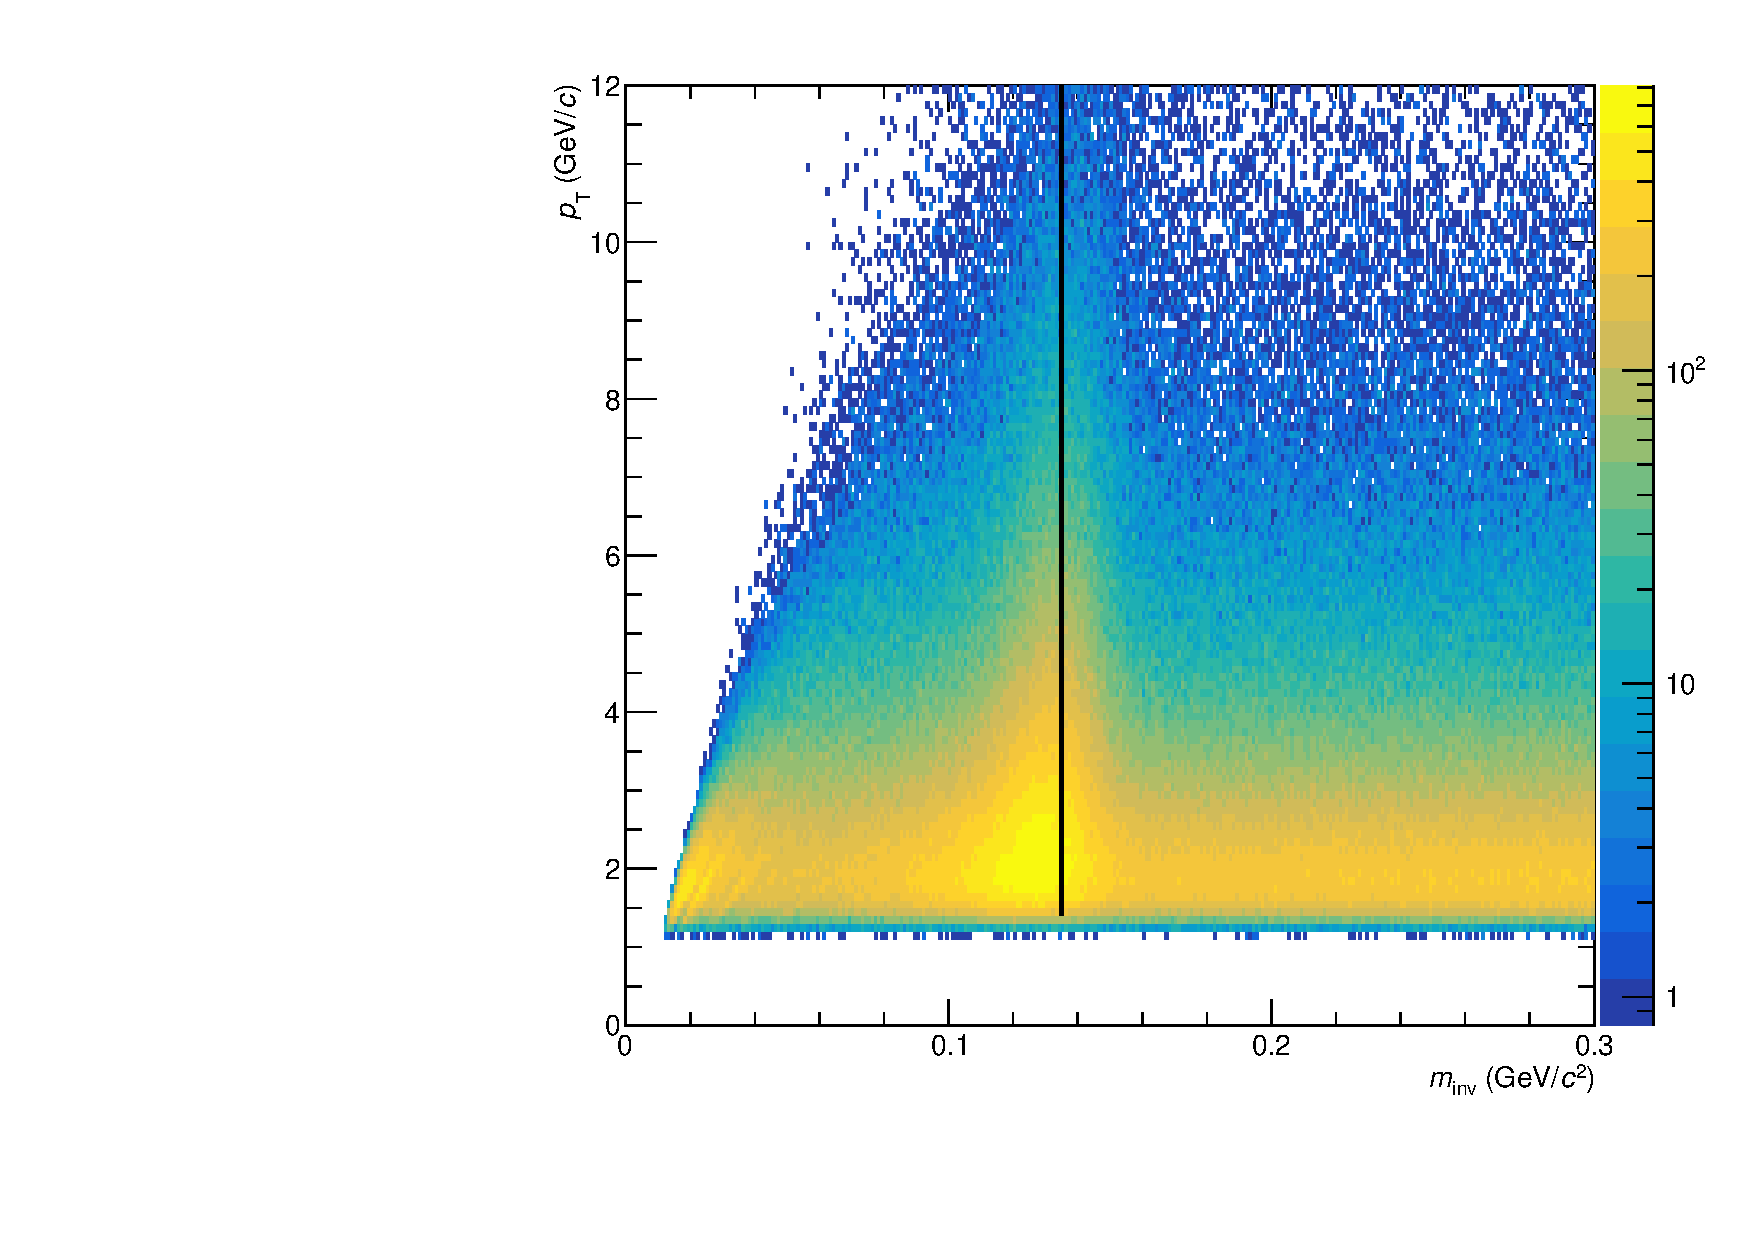
\includegraphics[width=.7\linewidth]{hInvMass_pT_Signal.pdf}
\caption{$p_\text{T}$ und $m_\text{inv}$ als Funktion von der Anzahl von rekombinierten  Cluster-Paaren aus der gleichen Kollision.
Die rote Linie liegt bei $m_{\text{inv}}\approx0\,135\text{ GeV/}c^{2}$, was in etwa der $\pi^{0}$ Masse entspricht, wo eine deutliche Häufung der Einträge sich abzeichnet.
Die schwarzen Linien stellen die Grenzen der $p_{\text{T}}$-Intervalle dar.}
\label{figInvMassPt_a}
\end{figure}
Um $\pi^{0}$ messen zu können, werden durch Kombinationen der Photonenkandidaten die invariante Masse und der Transversalimpuls nach Gleichungen \ref{eq_invmass} und \ref{eq_pt} bestimmt.
Da die Information, ob und welche Photonenkandidaten von dem Zerfall eines $\pi^{0}$ stammen fehlt, werden alle Photonenkandidaten eines \textit{events} paarweise mit einander kombiniert.
Dieses Vorgehen wird als \textit{same event method} bezeichnet.
Abbildung \ref{figInvMassPt_a} zeigt die Anzahl der Kombinationen in Abhängigkeit der invarianten Masse $m_{\text{inv}}$ und des Transversalimpulses $p_{\text{T}}$.
Durch die paarweise Kombination aller Photonenkandidaten eines \textit{Events} gibt es sowohl Kombinationen von Photonenkandidaten, die aus dem Zerfall eines $\pi^{0}$ stammen, als auch Photonenkandidaten, die nicht über den Zerfall eines $\pi^{0}$ zusammenhängen.
Die Summe aller Paare von Photonenkandidaten, die aus einem Zerfall eines $\pi^{0}$ kommen, wird als Signal bezeichnet.
Es zeichnet sich eine Häufung der Datenpunkte um $m_{\text{inv}}\approx 0\,135\text{ GeV}/c^{2}$, also um die Masse von $\pi^{0}$, ab.
Dieser Häufung liegen vor allem Kombinationen zusammengehöriger Photonenkandidaten zugrunde.
Aufgrund der Anforderung an den Öffnungswinkel gibt es bei kleinem $m_{\text{inv}}$ keine Datenpunkte.
Mit ansteigendem $p_{\text{T}}$ steigt der Wert von $m_{\text{inv}}$ für den kleinsten rekombinierten Datenpunkt.
Das führt dazu, dass mit steigendem $p_{\text{T}}$ ab einem bestimmten Punkt immer mehr Signal ausgeschlossen wird.
\newline
Die $p_{\text{T}}$-Abhängigkeit der Anzahl der $\pi^{0}$ weist auf unterschiedliche physikalische Effekte und Prozesse hin.
Deshalb wird die Verteilung aus Abbildung \ref{figInvMassPt_a} in einzelne $p_{\text{T}}$-Intervallen analysiert.
Die Intervalle werden so gewählt, dass sie möglichst klein sind, während die statistischen Unsicherheiten nicht zu groß werden.
\begin{figure}[tbp]
\centering
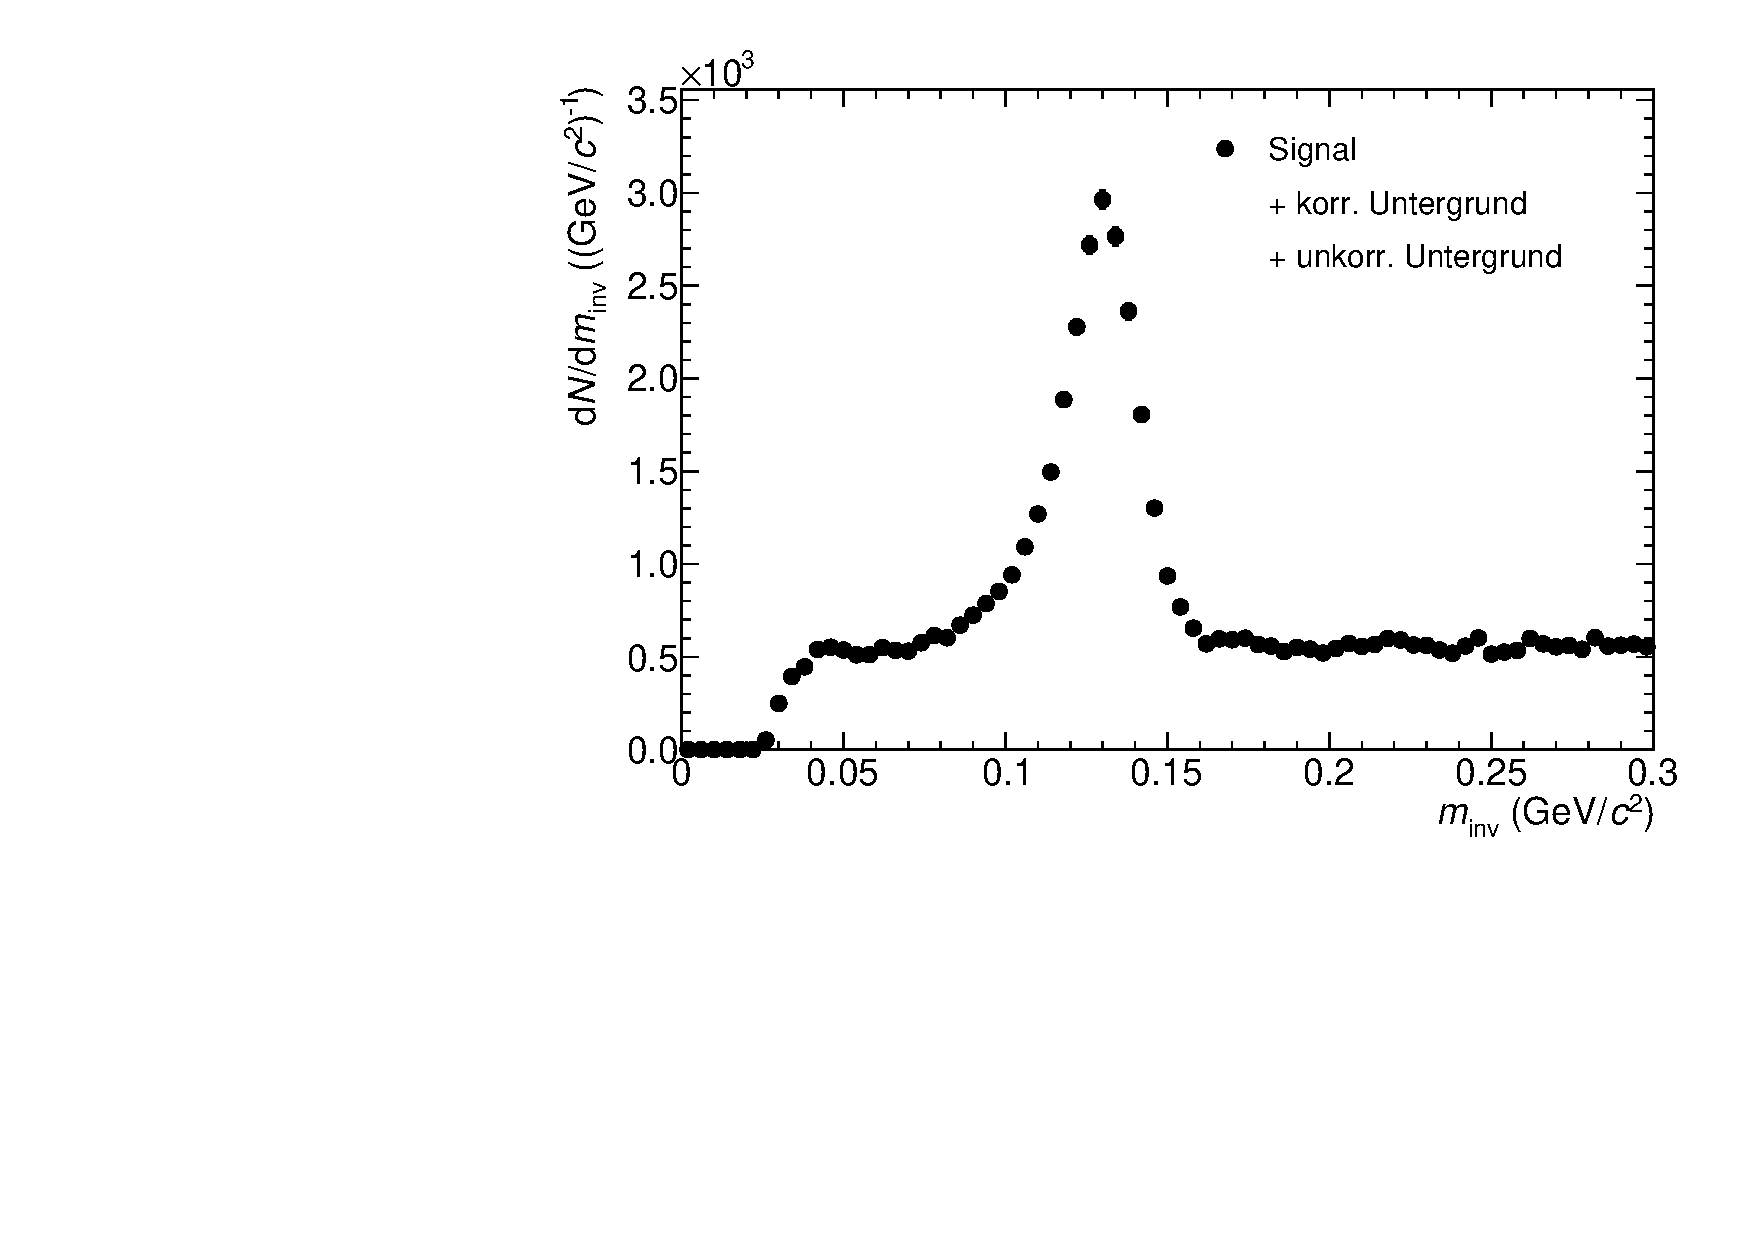
\includegraphics[width=.75\linewidth]{hSignalPlusBkg.pdf}
\caption{Projektion von Abbildung \ref{figInvMassPt_a} im $p_{\text{T}}$-Intervall $(3,2 - 3,4) (\text{GeV/}c)$. Es ist ein deutlicher Peak um $m_{\pi^{0}} \approx 0\,135\text{ GeV/}c^{2}$ zu erkennen, aber auch Untergrund, da das Signal zu höheren Massen gaußförmig abklingen sollte. Bei $m_{\text{inv}} < m_{\pi^{0}}$ kann Signal vorliegen, das aus konvertierten Photonen besteht, weshalb eine Aussage über die Form, beziehungsweise den Untergrund dort schwer möglich ist.}
\label{figSignalPlusBkg}
\end{figure}
\newline
Abbildung \ref{figSignalPlusBkg} zeigt eine Verteilung der invariante Massen in einem $p_{\text{T}}$-Intervall von $(3\,2 - 3\,4)(\text{GeV}/c)$.
Die zuvor beschriebene Anhäufung von Datenpunkten in Abbildung \ref{figInvMassPt_a} zeigt sich auch hier deutlich und wird im Folgenden als Peak bezeichnet.
Der Peak besteht wie oben erwähnt hauptsächlich aus richtig rekombinierten $\pi^{0}$.
Neben dem Signal besteht die Verteilung in Abbildung \ref{figSignalPlusBkg} noch aus sogenanntem Untergrund, der in zwei Teile unterteilt wird, den kombinatorischen oder auch unkorrelierten Untergrund und dem korrelierten Untergrund.
Dem korrelierten Untergrund hingegen liegen paarweise Kombinationen von Photonenkandidaten zugrunde, zwischen denen eine Korrelation besteht.
Das heißt, dass die Photonenkandidatenpaare nicht aus dem Zerfall eines $\pi^{0}$ stammen, aber über einen anderen Zerfall zusammenhängen.
Durch die paarweise Kombination unkorrelierter Photonenkandidaten, also solcher, die nicht aus einer Zerfallskette stammen, entsteht der unkorrelierte Untergrund.
\newline
Im folgenden Abschnitt wird eine Methode zur Abschätzung des unkorrelierten Untergrunds vorgestellt. 